\section{Weight and activation compression}
\label{sec:weights}

\subsection{Affine quantization}

Affine quantization~\citep{jacob2018quantization} maps a real weight \(x\) to a \(b\)-bit integer code
\begin{equation}
  q = \mathrm{clip}\!\left(\mathrm{round}\!\left(\tfrac{x}{s}+z\right),\, 0,\, 2^{b}-1\right),
  \qquad
  \hat{x} = s\,(q-z),
\end{equation}
with scale \(s\) and zero-point \(z\), typically shared by a group of \(G\) weights (e.g.\ 64 or 128). Group-wise scales keep dynamic range honest when a tensor has outliers. At inference, kernels dequantize on the fly or compute in low precision so a full FP16 copy is never materialized. GPTQ was motivated by 175B-class models that could not fit on a single GPU~\citep{frantar2022gptq}; the same math now makes 8B models comfortable on a laptop---an inversion of the original constraint that is exactly the everyday-device story.

\subsection{Post-training methods for LLMs}

\textbf{GPTQ}~\citep{frantar2022gptq} quantizes weights column-by-column, using a Hessian-aware update so remaining weights compensate for rounding error. \textbf{AWQ}~\citep{lin2023awq} identifies activation-salient channels and protects them so aggressive 4-bit quantization does not destroy the directions the network actually uses. \textbf{LLM.int8()}~\citep{dettmers2022llmint8} keeps outlier features in higher precision during 8-bit matmul. \textbf{SmoothQuant}~\citep{xiao2023smoothquant} migrates quantization difficulty from activations into weights, enabling W8A8-style pipelines. \textbf{OmniQuant}~\citep{shao2024omniquant} learns quantization parameters. Rotation / incoherence methods---QuaRot~\citep{ashkboos2024quarot}, SpinQuant~\citep{che2024spinquant}, QuIP\#~\citep{tseng2024quip}---make weights easier to quantize by changing basis. Additive residual codebooks (AQLM~\citep{egiazarian2024aqlm}) and sparse-quantized hybrids (SpQR~\citep{frantar2023spqr}, SqueezeLLM~\citep{kim2023squeezellm}) isolate a tiny high-precision outlier set. QServe~\citep{lin2024qserve} pushes a W4A8KV4 co-design into a serving engine.

In deployed local stacks, practitioners usually \emph{load} a pre-quantized checkpoint (GPTQ/AWQ/GGUF/MLX-community) rather than calibrating at serve time. Bit width \(b_w \in \{16,8,4,2\}\) is then a first-class serving knob. Empirically, \textbf{4-bit is the default sweet spot on unified-memory laptops}: 8-bit still spends too much DRAM for a daily driver; 2-bit frequently shows quality cliffs (Section~\ref{sec:empirical}).

\subsection{Activation quantization, mixed precision, pruning, distillation}

Activation quantization (W8A8, W4A8) matters when GEMM is compute-bound or when activation RAM dominates---more common in prefill and large-batch serving than in single-stream decode. Mixed precision (AMP) keeps accumulators in FP32 while storing weights in FP16/BF16; it is the default, not an extra flag, in most GPU stacks.

Pruning~\citep{han2015deep,frantar2023sparsegpt,ma2023llmpruner} removes weights. Unstructured sparsity needs specialized kernels to beat dense 4-bit GEMM on a laptop; structured (channel/head) pruning is easier to serve but harder to keep accurate. Knowledge distillation~\citep{hinton2015distilling,sanh2019distilbert} produces a smaller student: it is a \emph{different model}, not a runtime switch, but it is often the highest-leverage ``optimization'' if a 1--3B student meets the product bar---the Phi/TinyLlama/OpenELM bet~\citep{abdin2024phi3,zhang2024tinyllama,mehta2024openelm}.

\section{KV cache and context memory}
\label{sec:kv}

\subsection{Why the cache exists}

Scaled dot-product attention~\citep{vaswani2017attention} is
\begin{equation}
  \mathrm{Attention}(Q,K,V)=\mathrm{softmax}\!\left(\frac{QK^{\top}}{\sqrt{d_h}}\right)V.
\end{equation}
Recomputing \(K,V\) for the entire history at every decode step would repeat \(O(T)\) work per token. Caching per-layer \(K\) and \(V\) makes decode \(O(1)\) cache appends plus attention against the stored history. Equation~\eqref{eq:kv} then grows linearly in \(T\).

On a 24\,GB machine with 4-bit 8B weights ($\approx 5$\,GB), the cache is a rounding error at \(T=640\) and a second-class citizen that becomes first-class at long RAG, multi-turn agents, or (in servers) many concurrent sequences. Short-chat A/B tests that ``prove KV quant does nothing'' are measuring the wrong \(T\).

\subsection{Fewer KV heads}

Multi-query attention~\citep{shazeer2019mqa} shares one KV head across query heads. Grouped-query attention~\citep{ainslie2023gqa} interpolates, with \(H_{\mathrm{kv}} \ll H_q\). This is an \emph{architectural} reduction of \(M_{\mathrm{KV}}\) and of cache bandwidth. It explains why two 7B models can have very different long-context RAM slopes, and why Llama-3-class GQA is so friendly to laptops.

\subsection{Quantizing the cache}

KV quantization stores cached \(K,V\) at \(b_{\mathrm{kv}} < 16\) (commonly 8, 4, or even 2). It is independent of \(b_w\). KIVI~\citep{liu2024kivi} uses asymmetric 2-bit KV without fine-tuning. KVQuant~\citep{hooper2024kvquant} targets million-token contexts. Quality impact is usually smaller than aggressive weight quantization because each decode step only \emph{reads} the cache rather than using it as the model's entire knowledge. On-device, enable it as insurance once 4-bit weights have created headroom---especially on 16\,GB machines with less slack for RAG.

\subsection{Paging, prefix reuse, eviction, and sparsity}

\textbf{PagedAttention}~\citep{kwon2023vllm} stores KV in non-contiguous blocks so a serving engine can pack many sequences (Figure~\ref{fig:paged}). A laptop running one chat does not need a pager; a laptop running a local multi-user \texttt{llama-server} does. \textbf{Prefix / prompt caching} reuses KV for a repeated system prompt or RAG template: the first request pays prefill, later requests skip it. This is one of the highest-ROI everyday-device tricks and the local analogue of a provider's prompt cache.

\textbf{Eviction} drops tokens believed unimportant: H\(_2\)O keeps heavy hitters~\citep{zhang2023h2o}; StreamingLLM keeps an attention sink plus a sliding window~\citep{xiao2024streamingllm}; SnapKV~\citep{li2024snapkv} and Quest~\citep{tang2024quest} select what to keep given the query; DuoAttention~\citep{xiao2024duoattention} splits retrieval and streaming heads. Sliding-window attention (Mistral-style) bounds KV by construction~\citep{mistral2023}. These trade exact long-range attention for a bounded RAM envelope---exactly the phone/laptop deal.

\begin{figure}[t]
  \centering
  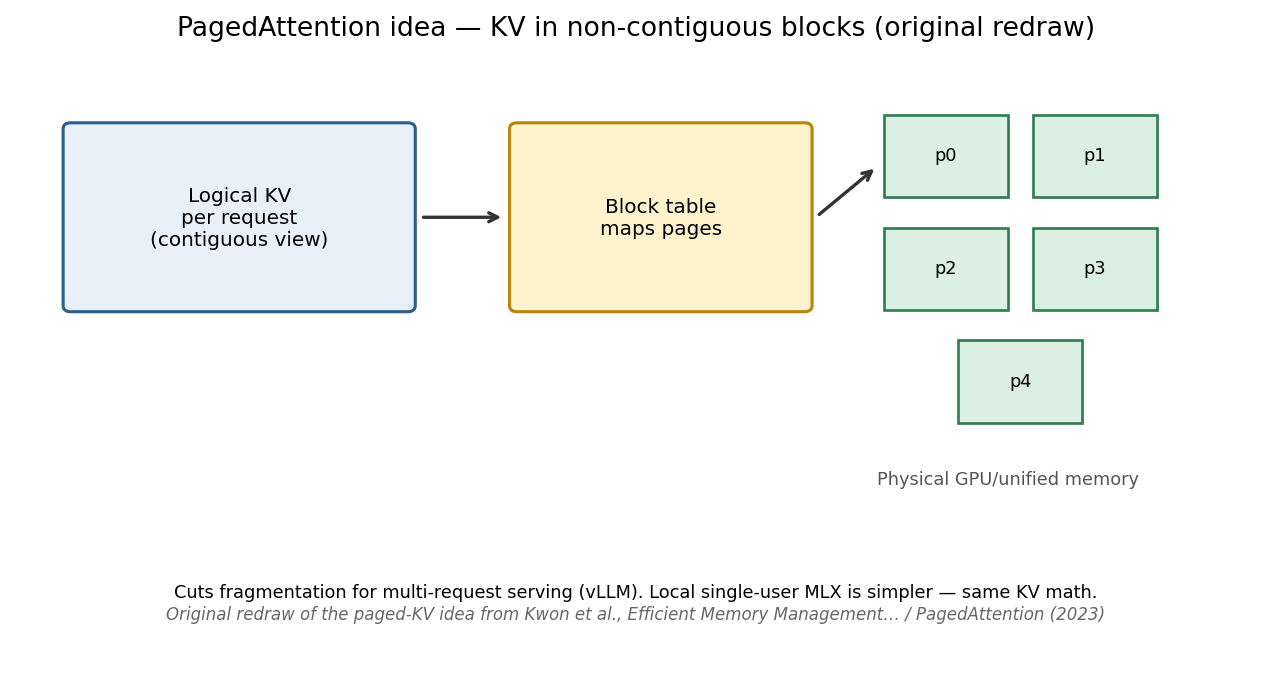
\includegraphics[width=0.92\linewidth]{figures/paged_attention.png}
  \caption{Paged KV (redraw after Kwon et al., 2023). Multi-user serving pages the cache; a daily-driver laptop is the single-tenant cousin of the same memory problem.}
  \label{fig:paged}
\end{figure}

\section{Attention kernels and prefill}
\label{sec:prefill}

Naive attention materializes \(S \in \mathbb{R}^{n \times n}\) per head. At \(n=2048\) and FP16 that is already \(\approx 8\)\,MB per head per layer. FlashAttention~\citep{dao2022flashattention} tiles \(Q,K,V\) through on-chip SRAM, uses an online softmax~\citep{milakov2018online}, and never writes the full score matrix to HBM. FlashAttention-2/3 improve parallelism and low-precision paths~\citep{dao2023flashattention2,dao2024flashattention3}. On Apple Silicon, MLX implements tiled Metal attention internally; user code rarely toggles a ``Flash'' flag. The user-visible leftover knob is often \textbf{chunked prefill} (prefill step size \(C\))~\citep{agrawal2023sarathipreprint,agrawal2024sarathi}: smaller \(C\) lowers peak activation memory; larger \(C\) often lowers TTFT when the device is under-occupied.

Long-prompt prefill is where everyday RAG dies. MInference~\citep{jiang2024minference} sparsifies prefill attention dynamically. Sparse and local attention~\citep{child2019sparse,beltagy2020longformer} reduce the \(O(n^2)\) term by restricting the pattern. State-space models~\citep{gu2023mamba} change the architecture. Rotary embeddings~\citep{su2024rope} and YaRN~\citep{peng2023yarn} extend usable context without a full pretrain; they do not by themselves reduce \(M_{\mathrm{KV}}\).

On a MacBook, the first prefill optimization is still application-level: retrieve fewer chunks (Section~\ref{sec:app}). The second is prefix cache. The third is kernels and \(C\).

\section{Decode-time algorithms}
\label{sec:decode}

\subsection{Speculative decoding}

Baseline decode costs \(\approx T_g \cdot \tau_t\) where \(\tau_t\) is one target-model forward. Speculative decoding~\citep{leviathan2023speculative,chen2023speculative} uses a cheap draft to propose \(k\) tokens; the target verifies them in one parallel forward and accepts a prefix of length \(m \le k\) under a rejection-sampling rule that preserves the target distribution (Figure~\ref{fig:spec}).

Let \(\alpha\) be the per-token acceptance probability. Wall-clock speedup requires \(\tau_d \ll \tau_t\) and high \(\alpha\). If the draft is a poor match, one still pays \(\tau_d + \tau_{\mathrm{verify}}\) and can \emph{lose} throughput---we measure this on Llama~3.1~8B (Section~\ref{sec:empirical}). Medusa~\citep{cai2024medusa} attaches extra heads to the target instead of a second model (attractive on phones where loading two graphs hurts). EAGLE~\citep{li2024eagle} drafts at the feature level. SpecInfer~\citep{miao2024specinfer} uses token trees. Lookahead and blockwise methods~\citep{chen2021lookahead,stern2018blockwise,spector2023rest} and Jacobi-style parallel decoding~\citep{santilli2023jacobidecoding} are related. Deja Vu~\citep{liu2024dejavu} skips compute via contextual sparsity.

On everyday devices speculation is a \emph{fourth} lever: it needs the RAM that 4-bit weights just freed, a tokenizer-compatible draft (0.5B--1B class), and a kill-switch when \(\alpha\) drops. CUDA graphs / Metal capture replay a static decode graph and help small-batch latency; they are complementary, not a substitute for bits.

\begin{figure}[t]
  \centering
  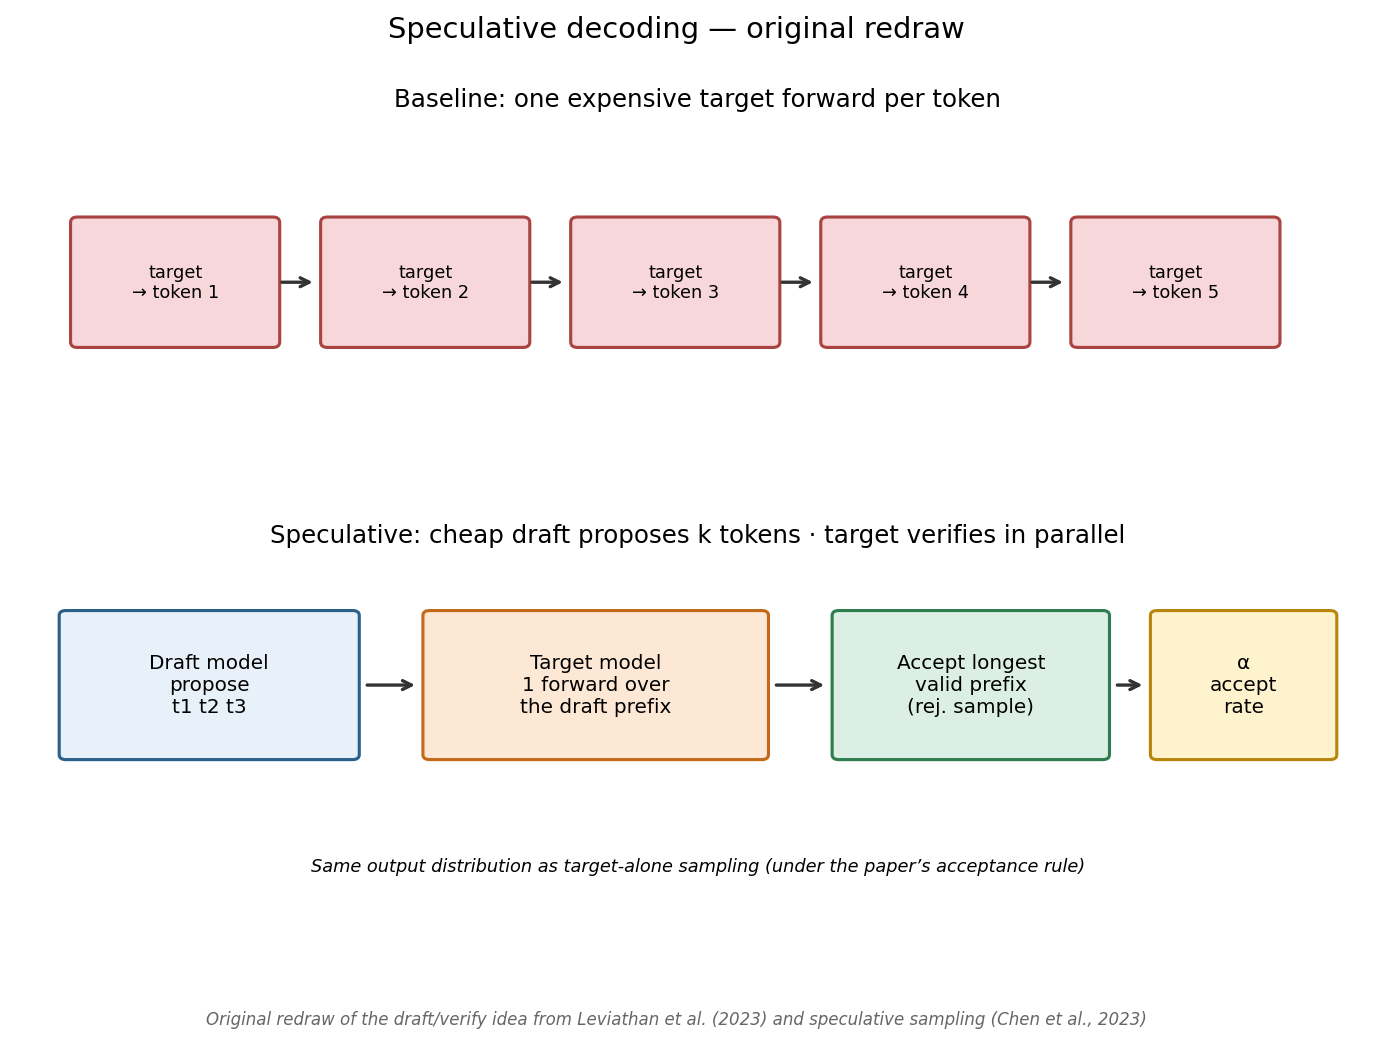
\includegraphics[width=0.92\linewidth]{figures/speculative.png}
  \caption{Speculative decoding (redraw after Leviathan et al.\ and Chen et al.). Speedup tracks acceptance \(\alpha\) and draft cost, not merely the presence of a draft---critical on memory-tight laptops.}
  \label{fig:spec}
\end{figure}

\section{Batching, scheduling, and disaggregation}
\label{sec:serving}

Local \texttt{generate()} loops are single-stream. Production serving is not. We include this family because (i)~the same human may later run \texttt{llama-server} for a household, and (ii)~papers in this family invented paging and chunked prefill that local stacks now expose as flags.

\textbf{Static batching} waits to fill a batch of size \(B\). \textbf{Continuous batching} (iteration-level scheduling)~\citep{yu2022orca,kwon2023vllm} mixes prefill of new requests with decode of in-flight ones. \textbf{Chunked prefill} in Sarathi-Serve~\citep{agrawal2024sarathi} piggybacks decode tokens alongside partial prefills. \textbf{Disaggregated prefill/decode}~\citep{patel2024splitwise,aminabadi2024distserve} places the two phases on different pools. SGLang~\citep{zheng2024sglang} adds a radix cache and structured generation. Request scheduling adds SLOs and preemption.

On a daily-driver laptop with one user, continuous batching does almost nothing. On a Mac mini serving a family, it suddenly does. The mistake is cargo-culting vLLM flags before the model fits beside Safari.

\section{Parallelism}
\label{sec:parallel}

When one device cannot hold the model, inference reuses training sharding: tensor parallel~\citep{shoeybi2019megatron,narayanan2021efficient}, pipeline parallel~\citep{huang2019gpipe}, expert parallel for MoE~\citep{fedus2022switch,lepikhin2021gshard,jiang2024mixtral,yi2023edgemoe}, and data parallel for large batches. Consumer Macs almost never expose multi-GPU tensor parallel for LLMs; the relevant decision is ``does this dense 70B fit in unified memory at 4-bit?'' (usually no on 24\,GB; sometimes yes on 128\,GB Ultra). A single consumer NVIDIA GPU plus CPU offload~\citep{sheng2023flexgen,song2024powerinfer,alizadeh2024llm} is the PC analogue. EdgeMoE~\citep{yi2023edgemoe} specifically targets on-device MoE.

\section{Architecture and model-size choices}
\label{sec:arch}

The highest-leverage ``optimization'' on a small machine is sometimes a smaller model. Memory~\eqref{eq:weights} and bandwidth-bound decode~\eqref{eq:roofline} both scale with \(N\). A dense 0.5B 4-bit model and a dense 8B 4-bit model can differ by an order of magnitude in tokens/s on the same laptop (Section~\ref{sec:empirical}). Phi-3~\citep{abdin2024phi3}, TinyLlama~\citep{zhang2024tinyllama}, OpenELM~\citep{mehta2024openelm}, MobileLLM~\citep{liu2024mobilellm}, Gemma~2 2B~\citep{team2024gemma2}, and Llama~3.2 1B/3B exist because of that curve. Mixture-of-experts~\citep{jiang2024mixtral,liu2024deepseek} offers more total parameters at a smaller active-FLOP budget, at the cost of a larger memory floor---painful on 16\,GB, interesting on 64\,GB. Long-context variants inflate \(T\) in~\eqref{eq:kv} and prefill cost. Instruction-tuned versus base checkpoints should be held fixed in systems benchmarks; they are not speed knobs.

\section{Adapters}
\label{sec:lora}

LoRA~\citep{hu2022lora} injects low-rank updates \(BA\) into frozen weights. QLoRA~\citep{dettmers2023qlora} fine-tunes those adapters on a quantized base---the reason a laptop can specialize an 8B model overnight. At inference, each adapter adds a small extra GEMM and RAM. Multi-LoRA serving swaps adapters per request; that is a server problem. For a single local user, one LoRA is usually noise compared with \(b_w\), and it is how ``my coding style'' becomes an on-device file rather than a cloud fine-tune.

\section{Compilation, kernels, and runtimes}
\label{sec:runtime}

Graph compilation (\texttt{torch.compile}, \texttt{mlx.compile}, XLA, TensorRT-LLM~\citep{nvidia2024trtllm}, MLC~\citep{mlcllm}) fuses ops and specializes shapes. Quantized matmul kernels determine whether 4-bit is actually faster than FP16 or merely smaller. CPU/disk offload~\citep{sheng2023flexgen,alizadeh2024llm} runs models that do not fit, at a large bandwidth penalty. Memory-mapping weights from SSD reduces cold-start RAM spikes.

Local runtimes illustrate that \emph{the same bit width is not the same system}:

\begin{itemize}[leftmargin=*,itemsep=2pt]
  \item \textbf{MLX / mlx-lm}~\citep{mlx2023,mlxlm2023}: Metal-native arrays, Hugging Face \texttt{mlx-community} checkpoints, Python harnesses---the path we measure.
  \item \textbf{llama.cpp / GGUF}~\citep{llamacpp,gguf}: C/C++, Metal/CUDA/CPU, community GGUF quants (Q4\_K\_M, Q8\_0, \ldots). The default engine behind much of local-LLM culture.
  \item \textbf{Ollama}~\citep{ollama}: distribution and UX over llama.cpp-class engines.
  \item \textbf{MLC LLM}~\citep{mlcllm}: TVM compilation across GPU/NPU/CPU.
  \item \textbf{ExecuTorch}~\citep{executorch}: mobile/edge PyTorch.
  \item \textbf{PowerInfer}~\citep{song2024powerinfer}: hot-neuron GPU + cold-neuron CPU on a consumer PC.
\end{itemize}

Fair comparison requires matched prompts, generation length, and a comparable quant \emph{tier} (FP16 vs.\ F16 GGUF; 4-bit MLX vs.\ Q4\_K\_M), not matched marketing names.

\section{Application-level inference}
\label{sec:app}

Not every latency problem belongs inside the model---especially on everyday devices, where the user controls the prompt.

Retrieval-augmented generation~\citep{lewis2020rag} can \emph{increase} TTFT by stuffing thousands of tokens into \(T_p\). The correct optimization is often ``retrieve less'' or ``rerank then truncate.'' Prefix caches (Section~\ref{sec:kv}) absorb repeated templates. Semantic prompt caches reuse prior completions. Constrained / structured decoding~\citep{willard2023outlines,zheng2024sglang} masks logits toward JSON or grammars; it adds CPU work per token. Early-exit and confidence stopping~\citep{schuster2022confident} cut \(T_g\). Nucleus and temperature~\citep{holtzman2020nucleus} are quality knobs with mild speed effects. Tool/function calling~\citep{alizadeh2024llmcompiler} is an application graph; on a laptop, serial tool loops dominate wall-clock more than GEMM.

The daily-driver heuristic: \textbf{every token you do not retrieve is a token you do not prefill.}
